\documentclass[12pt,a4paper]{article}
\pdfminorversion=7

\usepackage{preamble}

\addbibresource{refs.bib}

\begin{document}

\pagenumbering{Alph}  % Numeración alfabética para titlepage (evita duplicados)
\begin{titlepage}
	\vspace*{-2cm}
	% --- LOGOTIPOS (ALINEADOS ARRIBA, IZQUIERDA Y DERECHA) ---
	\noindent
	
\includegraphics[width=0.35\textwidth]{ule.jpg}
	\hfill
	
\includegraphics[height=2.5cm]{escudo-ingenierias.png}

	\vspace{0.2cm}

	% --- CUADRO AZUL PARA EL TÍTULO ---
	\begin{tcolorbox}[colback=maincolor,colframe=maincolor,arc=0pt,outer arc=0pt,grow to left by=3cm,grow to right by=3cm,fontupper=\color{white}]
		\centering
		\vspace{0.8cm}
		{\Huge \bfseries INSTALACIONES II}\\[0.4cm]
		{\Large PRÁCTICA DE PROTECCIÓN CONTRA INCENDIOS}
		\vspace{0.8cm}
	\end{tcolorbox}

	\vspace{0.5cm}
	\begin{center}
		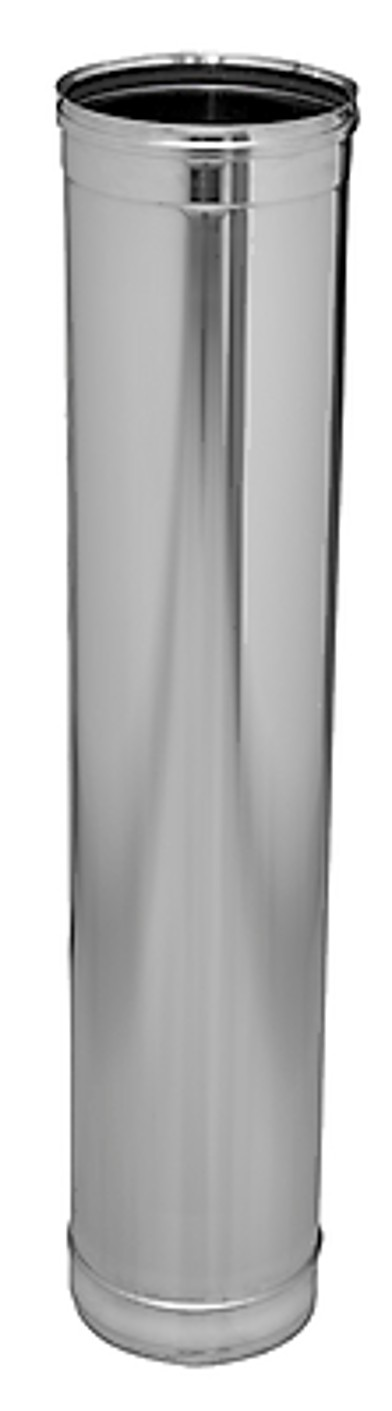
\includegraphics[height=9cm, keepaspectratio]{Figuras/chimenea_recta.jpg}
	\end{center}
	\vfill

	% --- AUTORES Y DATOS (ALINEADOS A LA DERECHA, SIN CUADRO) ---
	\begin{flushright}
		\large
		\begin{tabular}{@{}ll}
			\textbf{Grupo:}   & 1 \\ [5pt]
			\textbf{Autores:} & Alberto España Carrete   \\
                        & Carlos Fernández Palanca \\
                        & Rubén Modino López      \\
                        & Juan Diego Niño González \\ [5pt]
      		\textbf{Tutor:}   & José Luis Falagán Cavero
			
		\end{tabular}
	\end{flushright}

	\vspace{0.5cm}

	\begin{center}
    {\fontsize{16pt}{19pt}\LARGE(Junio, 2026)}
  	\end{center}
\end{titlepage}

\pagenumbering{roman}
\clearpage
\pagestyle{empty}

{
	\hypersetup{linkcolor=black}
	\tableofcontents
	\clearpage

	% --- Índice de figuras ---
	{
		\let\oldnumberline\numberline
		\renewcommand{\numberline}{\figurename~\oldnumberline}
		\listoffigures
		\phantomsection
		\addtocontents{toc}{\protect\cftpagenumbersoff{section}}
		\addcontentsline{toc}{section}{\listfigurename}
		\addtocontents{toc}{\protect\cftpagenumberson{section}}
	}
	\clearpage

}

\pagenumbering{arabic}
\pagestyle{contenido}
\section*{Resumen}
\phantomsection
\addcontentsline{toc}{section}{Resumen}

La memoria desarrolla el diseño y la comprobación hidráulica de una instalación de protección contra incendios para un edificio residencial, formada por una red de Bocas de Incendio Equipadas y una red de rociadores automáticos. El trabajo abarca la definición del trazado, la selección de equipos comerciales y la construcción de un modelo de cálculo tridimensional que permite verificar el comportamiento de presiones, caudales, velocidades y la reserva de agua.

El resultado principal es un diseño de instalación capaz de satisfacer simultáneamente las demandas de los puntos de consumo más desfavorables del edificio. El dimensionamiento del grupo de presión y de la reserva de agua en el aljibe garantiza el cumplimiento de los tiempos mínimos de autonomía y los niveles de presión requeridos. Las simulaciones hidráulicas confirman que tanto la Boca de Incendio Equipada crítica como el rociador automático más desfavorable operan con las presiones en boquilla necesarias para asegurar el correcto funcionamiento del sistema y el cumplimiento de la normativa de seguridad aplicable. En conjunto, la solución planteada queda técnicamente justificada, adjuntándose los cálculos complementarios, planos y especificaciones técnicas correspondientes.

\section{Introducción e objetivos}

\subsection{Contexto y Marco Normativo}

En el diseño arquitectónico y de ingeniería contemporáneo, la seguridad frente a incendios representa uno de los requerimientos más estrictos e ineludibles. En los edificios destinados a uso residencial colectivo, donde la densidad de ocupación y los tiempos de evacuación en caso de emergencia pueden elevar sustancialmente el riesgo para las vidas humanas, la implementación de medidas eficaces de protección activa contra incendios resulta indispensable. La protección activa comprende todos aquellos equipos y sistemas instalados con el objeto de detectar la presencia de fuego, controlar su propagación radial o vertical, y proceder a su mitigación o extinción definitiva. La funcionalidad de estos sistemas se divide fundamentalmente entre la intervención temprana manual y la supresión autónoma e inmediata.

Las Bocas de Incendio Equipadas (BIE) representan el exponente clásico de los sistemas de protección activa de accionamiento manual y primera intervención. Compuestas estructuralmente por una manguera, un soporte giratorio, una válvula de paso y una boquilla lanza con posibilidad de regular el chorro de agua, permiten a los ocupantes del propio edificio o a los equipos de primera intervención desplegar una línea de agua presurizada para combatir el fuego en su fase de gestación o desarrollo inicial. Su flexibilidad radica en el control directo del chorro de agua hacia el foco del incendio, lo que maximiza la eficiencia en la aplicación del agente extintor y permite enfriar las superficies adyacentes de manera dirigida. No obstante, al depender de la acción humana para su puesta en marcha y manejo, su efectividad está sujeta a la presencia física de personas capacitadas y a las condiciones de visibilidad y temperatura ambiental en el sector afectado.

Por el contrario, los sistemas de rociadores automáticos (\textit{sprinklers}) constituyen sistemas autónomos y automáticos de supresión de incendios que no requieren de la intervención humana directa. Estos emisores están distribuidos estratégicamente a nivel de techo y permanecen cerrados por medio de un elemento térmicamente sensible ---como un bulbo de vidrio que contiene un líquido expansible al calor o un fusible de aleación eutéctica---. Cuando la columna de gases calientes de un incendio incide sobre el rociador y este alcanza una temperatura predeterminada de activación, el elemento fusible se rompe o funde, liberando el obturador y permitiendo la descarga inmediata de un patrón de agua pulverizada en forma de parábola sobre el foco ígneo. Esta respuesta autónoma no solo controla localmente el incendio y limita el incremento de temperatura ambiental en el recinto, sino que además mitiga la generación de humos tóxicos, facilitando las labores de evacuación y protegiendo la integridad estructural del edificio.

El marco normativo nacional español impone una rigurosa estructura técnica y prestacional para garantizar la idoneidad y fiabilidad de estos sistemas de extinción hidráulica. El Código Técnico de la Edificación, en su Documento Básico de Seguridad en caso de Incendio (CTE DB-SI), actúa como la norma marco que define las exigencias mínimas de seguridad en el territorio español, determinando en qué condiciones de uso, altura de evacuación o superficie es obligatoria la instalación de determinados elementos de protección activa. Paralelamente, el Reglamento de Instalaciones de Protección Contra Incendios (RIPCI, aprobado por el Real Decreto 513/2017) gobierna las condiciones de diseño, instalación, mantenimiento preventivo y características de calidad de los componentes de las instalaciones \parencite{CTE_DBSI,RIPCI_2017,RIPCI_GUIA_2022}. 

La relevancia técnica de este reglamento radica en que obliga a que todo elemento instalado disponga de una certificación de conformidad con las normas armonizadas europeas. En el caso de las Bocas de Incendio Equipadas con manguera semirrígida (generalmente de diámetro nominal de veinticinco milímetros por su mayor facilidad de manejo), el diseño hidráulico y de componentes se rige por la norma UNE-EN 671-1, que fija los requisitos de caudal mínimo de boquilla en función de la presión dinámica de entrada. Por su parte, la norma de referencia para el diseño, cálculo e instalación de los rociadores automáticos es la UNE-EN 12845, la cual establece de manera pormenorizada las demandas de densidad de diseño (expresada en litros por minuto y metro cuadrado), las áreas de operación de cálculo correspondientes según la clasificación del riesgo (como el Riesgo Ligero o el Riesgo Ordinario) y la autonomía mínima necesaria de la reserva de agua para garantizar una operación hidráulica fiable en condiciones extremas \parencite{UNE_EN_671_1,UNE_EN_12845}.

Para ilustrar de forma práctica la inserción de estos sistemas dentro del esquema de protección activa, \cref{fig:ipci} ofrece un diagrama conceptual de la tipología de las instalaciones de protección contra incendios consideradas. Por su parte, \cref{fig:bie_fun,fig:rociador_fun} ejemplifican, respectivamente, una Boca de Incendio Equipada en fase de operación manual y un rociador automático activado por su elemento termosensible en una fase autónoma de control de incendio.

\begin{figure}[H]
	\centering
	
\includegraphics[width=0.6\textwidth]{IPCI.png}
	\caption{Contexto general de las instalaciones de protección contra incendios. Fuente: Elaboración grupal.}
	\label{fig:ipci}
	\vspace{0.1cm}
\end{figure}

\begin{figure}[H]
	\centering
	
\includegraphics[width=0.5\textwidth]{BIE_en_funcionamiento.png}
	\caption{Boca de Incendio Equipada de manguera semirrígida en funcionamiento. Fuente: Elaboración grupal.}
	\label{fig:bie_fun}
	\vspace{0.1cm}
\end{figure}

\begin{figure}[H]
	\centering
	
\includegraphics[width=0.5\textwidth]{Rocioador_en_funcionamiento.png}
	\caption{Rociador automático en funcionamiento por activación termosensible. Fuente: Elaboración grupal.}
	\label{fig:rociador_fun}
	\vspace{0.1cm}
\end{figure}

El objetivo primordial del presente proyecto consiste en capacitar al proyectista en el diseño integral, dimensionamiento hidráulico y verificación reglamentaria de una instalación de protección contra incendios para un edificio residencial colectivo. El enfoque del estudio no se limita a un mero cálculo mecánico, sino que persigue el análisis crítico del comportamiento hidráulico del agua bajo diversas condiciones de demanda simultánea. Para alcanzar este propósito general, se establecen los siguientes objetivos específicos:

\begin{itemize}
	\item Diseño geométrico e hidráulico de la red de BIEs.
	\item Dimensionamiento y distribución del sistema de rociadores automáticos.
	\item Verificación reglamentaria.
	\item Optimización y resolución de singularidades.
\end{itemize}

\section{Metodología}

El diseño y cálculo hidráulico de la instalación combinada de protección contra incendios se ha desarrollado mediante una metodología de modelización tridimensional del edificio y simulación por computador. A partir de las hipótesis de diseño y los requisitos normativos aplicables, se ha construido un modelo matemático para analizar las presiones dinámicas, velocidades y caudales en los nudos del sistema, asegurando el cumplimiento de las condiciones de funcionamiento seguro.

\subsection{Datos introducidos en el programa}

El cálculo de la instalación hidráulica se realiza mediante un modelo numérico en el que se definen los elementos de la red mediante nudos y líneas. Los nudos representan conexiones físicas, derivaciones, cambios de dirección y los puntos terminales de consumo (Bocas de Incendio Equipadas y rociadores automáticos), así como la aspiración del depósito y el grupo de bombeo. Las líneas corresponden a los tramos de tubería caracterizados por su longitud real, material, diámetro nominal y diámetro interior \parencite{UNE_EN_12845}. 

Las bases de diseño hidráulico aplicadas en la simulación del sistema se rigen por coeficientes y parámetros de cálculo normalizados. Para las conducciones, fabricadas en acero al carbono sin soldadura, se define un coeficiente de rugosidad de Hazen-Williams de $C = 120$, conforme a las especificaciones de las tablas de producto y a las prescripciones de la norma UNE-EN 12845. El motor de cálculo del programa procesa las pérdidas de carga lineales basándose en esta formulación hidráulica, la cual es adecuada para fluidos a presión en materiales metálicos. Con el propósito de contabilizar de forma simplificada pero segura las pérdidas de carga secundarias provocadas por las uniones ranuradas, codos, derivaciones y válvulas de corte presentes en la red, se introduce un coeficiente global que incrementa en un \SI{20}{\percent} las pérdidas por rozamiento lineal a lo largo de toda la instalación \parencite{UNE_EN_12845}. 

A nivel dinámico, la velocidad máxima del fluido en los tramos se restringe a un límite técnico de \SI{10.0}{\meter\per\second} para prevenir el desgaste erosivo prematuro de las tuberías de acero y evitar fenómenos de inestabilidad hidráulica o golpe de ariete. En cuanto a los terminales de descarga, se configuran dos escenarios operacionales bajo la hipótesis de simultaneidad y clasificación de Riesgo Ordinario 1 (RO1) regulada por la UNE-EN 12845. Esto impone una autonomía mínima de diseño de \SI{60}{\minute} tanto para el sistema de rociadores como para el de Bocas de Incendio Equipadas \parencite{RIPCI_GUIA_2022,UNE_EN_12845}. 

Para las Bocas de Incendio Equipadas de manguera semirrígida de veinticinco milímetros de diámetro nominal (BIE 25), el Reglamento de Instalaciones de Protección Contra Incendios y la norma UNE-EN 671-1 establecen una presión residual mínima en boquilla (punta de lanza) de \SI{2.0}{\bar} para asegurar un alcance de chorro y caudal de descarga mínimos efectivos, fijándose asimismo una presión estática máxima de \SI{6.0}{\bar} a la entrada del armario de la BIE para proteger los componentes y garantizar la seguridad de manipulación de los operarios. Cualquier exceso eventual en nudos de cotas bajas del edificio se corrige localmente en obra incorporando válvulas reductoras de presión \parencite{RIPCI_GUIA_2022,UNE_EN_671_1}. 

Para los rociadores automáticos de cobertura extendida (modelo Tyco Series EC-11), la ficha técnica de producto establece una presión mínima residual de funcionamiento de \SI{0.83}{\bar}; sin embargo, debido a las restricciones de redondeo en la interfaz gráfica del software de cálculo empleado, este valor se introduce en el modelo con un valor nominal redondeado de \SI{0.8}{\bar}. El volumen de reserva conjunta y el dimensionamiento definitivo de la bomba y el aljibe se determinan a partir de estas restricciones hidráulicas para abastecer la demanda simultánea combinada del área hidráulica de diseño y los puntos de consumo críticos manuales \parencite{TYCO_EC11,UNE_EN_12845}.

El grupo de bombeo y la reserva de agua se calculan para satisfacer la demanda simultánea de los sistemas según las hipótesis de operación: el funcionamiento de las dos Bocas de Incendio Equipadas más desfavorables de forma simultánea y el funcionamiento del área de operación de rociadores definida.

\subsection{Topología del edificio y selección del esquema de instalación}

El edificio residencial objeto de estudio se compone de un perfil arquitectónico de cinco plantas sobre rasante destinadas a uso de viviendas colectivas y una planta de garaje-aparcamiento subterránea situada en sótano. El esquema hidráulico de protección contra incendios se unifica mediante una red común de alimentación por columna húmeda presurizada, gobernada de manera centralizada por un único grupo de presión de protección contra incendios emplazado en la planta de sótano, contiguo a un depósito o aljibe de reserva de agua común de gran capacidad.

Desde el grupo de bombeo de sótano, el caudal es impulsado en sentido ascendente a través de una columna montante vertical principal de acero al carbono que recorre el patinillo técnico del núcleo común de comunicaciones del edificio. Los diámetros de esta columna montante vertical están calculados y optimizados para atemperar las pérdidas de fricción y el coste material. Así, la montante se inicia en su base con un diámetro nominal de DN40 (\SI{40}{\milli\meter}), manteniéndose este diámetro intermedio a lo largo de las plantas de menor cota, y reduciéndose en su tramo superior a un diámetro de DN32 (\SI{32}{\milli\meter}) para alimentar las últimas viviendas a cota más elevada. A pesar del estrechamiento superior, la velocidad del fluido en la tubería vertical se estabiliza en un valor máximo de \SI{8.62}{\meter\per\second} ante la demanda combinada extrema, valor que respeta holgadamente el límite de erosión de \SI{10.0}{\meter\per\second} fijado en las bases de cálculo del programa.

A partir de esta columna montante común de distribución vertical, se realizan las derivaciones correspondientes por planta para alimentar de forma selectiva a los sistemas instalados:
\begin{enumerate}
	\item \textbf{Derivaciones de Bocas de Incendio Equipadas (BIEs)}: Consisten en derivaciones de diámetro DN32 (diámetro interior de \SI{36.0}{\milli\meter}) que conectan de forma individualizada el colector vertical con los armarios de Bocas de Incendio Equipadas empotrados en las zonas de distribución común (vestíbulos previos o pasillos de acceso a viviendas) de cada planta de cota residencial.
	\item \textbf{Derivaciones de rociadores automáticos}: Conectan la columna común con una red de distribución horizontal en ramales horizontales de acero que discurren bajo el falso techo de los pasillos comunes y de los interiores de las viviendas, reduciendo progresivamente su diámetro en función de la cercanía a los rociadores terminales individuales para optimizar las velocidades y presiones dinámicas de diseño.
\end{enumerate}

La relación espacial y topológica entre las cotas del edificio, las plantas y las líneas del modelo de cálculo se ilustra con las siguientes figuras de apoyo: \cref{fig:def_plantas} muestra la definición de plantas y cotas geométricas del edificio en el modelo, mientras que \cref{fig:perfil_plantas} representa la relación entre el perfil vertical, cotas y plantas del edificio.

\begin{figure}[H]
	\centering
	
\includegraphics[width=0.7\textwidth]{definicion_plantas.png}
	\caption{Definición de plantas y cotas geométricas del edificio en el modelo. Fuente: Elaboración grupal.}
	\label{fig:def_plantas}
	\vspace{0.1cm}
\end{figure}

\begin{figure}[H]
	\centering
	
\includegraphics[width=0.5\textwidth]{Perfil_Plantas.png}
	\caption{Relación entre perfil vertical, cotas y plantas del edificio. Fuente: Elaboración grupal.}
	\label{fig:perfil_plantas}
	\vspace{0.1cm}
\end{figure}

Los planos unifilares de la instalación en tres dimensiones y los detalles de perfil se incorporan en la documentación complementaria adjunta, recogida en \cref{anex:planos}.

\subsection{Justificación del trazado elegido}

El trazado de la instalación de protección contra incendios se justifica bajo criterios rigurosos de accesibilidad, continuidad hidráulica, simplificación de recorridos físicos y cobertura espacial completa del edificio, garantizando la seguridad en toda la planta construida:
\begin{itemize}
	\item \underline{Trazado de ramales y montantes}: La columna montante discurre por patinillos técnicos y conductos verticales comunes en zonas de escaleras y ascensores, lo que facilita las labores de mantenimiento preventivo, inspección visual reglamentaria e independiza los tramos principales del interior de las viviendas. Los ramales de distribución horizontal se canalizan bajo el falso techo desmontable en pasillos y zonas comunes, y a través de falsos techos fijos en las viviendas para no interferir con la estética de las dependencias residenciales.
	\item \underline{Alcance y cobertura de las bocas de incendio}: Los armarios de las Bocas de Incendio Equipadas se posicionan estratégicamente en los vestíbulos de distribución común de cada planta, inmediatamente contiguos a las vías de evacuación principales. La ubicación de estos armarios garantiza que, considerando una manguera semirrígida comercial de \SI{30}{\meter} de longitud nominal y un alcance físico proyectado del chorro de agua de lanza de al menos \SI{5}{\meter} (totalizando \SI{35}{\meter} de radio de acción geométrico), se cubra completamente y sin puntos ciegos toda la superficie útil del vestíbulo común, los accesos verticales y las viviendas completas de la planta residencial correspondiente.
	\item \underline{Distribución de la red de rociadores}: Los ramales horizontales de rociadores automáticos se ramifican bajo techo para cubrir todas las estancias de las viviendas residenciales. La superficie física total que cuenta con cobertura física protegida mediante la red de rociadores automáticos en la planta residencial es de exactamente \SI{270.88}{\meter\squared}. Esta superficie física instalada se desglosa geométricamente en dos viviendas simétricas de \SI{127.97}{\meter\squared} de superficie útil de distribución interior cada una, sumado al pasillo común y vestíbulo de acceso que aportan \SI{14.95}{\meter\squared}.
	\item \underline{Diferencia entre superficie física y área hidráulica activa}: Es fundamental aclarar en términos de ingeniería que esta superficie total protegida de \SI{270.88}{\meter\squared} corresponde al alcance físico constructivo total de las tuberías e inyectores instalados por planta, pero \textbf{bajo ninguna circunstancia representa el área de cálculo hidráulica activa}. En el cálculo y simulación hidráulica conforme a la UNE-EN 12845 para Riesgo Ordinario 1 (RO1), el motor del software solo activa simultáneamente el área de operation más desfavorable de rociadores en funcionamiento conjunto (en nuestro modelo, los 3 rociadores críticos activos representados por los nudos 140, 141 y 142). Esto permite dimensionar la bomba de incendios y el volumen de reserva con la máxima demanda de flujo puntual esperada y evitar un sobredimensionamiento desmesurado de la red colectora y grupos activos que harían la instalación inviable económicamente.
	\item \underline{Velocidades de circulación y pérdidas de carga}: El diseño hidráulico del trazado evita ramificaciones excesivas y busca recorridos lo más lineales posibles. Los diámetros de los ramales de distribución horizontal se dimensionan de forma decreciente hacia los terminales para equilibrar las pérdidas de carga y estabilizar las velocidades del agua por debajo de los \SI{10.0}{\meter\per\second} admisibles (con un valor pico de \SI{8.62}{\meter\per\second} en la montante reducida y velocidades inferiores en los ramales de viviendas), controlando el desgaste físico y maximizando la presión residual disponible en las boquillas de descarga.
\end{itemize}

La relación entre el trazado inicial, las derivaciones y los armarios de BIE queda detallada de forma gráfica en \cref{fig:inicio_tramos}, que ilustra el esquema inicial de trazado, tramo y ubicación de una Boca de Incendio Equipada en la red.

\begin{figure}[H]
	\centering
	
\includegraphics[width=0.45\textwidth]{Inicio_Tramo_y_BIE.png}
	\caption{Esquema del inicio de tramos y conexión de la Boca de Incendio Equipada en la red.}
	\label{fig:inicio_tramos}
	\vspace{0.1cm}
\end{figure}

\subsection{Equipos instalados y materiales de la instalación}

La instalación emplea equipos comerciales homologados y materiales que cumplen con los estándares de fabricación y resistencia exigidos por el RIPCI \parencite{RIPCI_2017,RIPCI_GUIA_2022}:
\begin{enumerate}
	\item \underline{Bocas de Incendio Equipadas (BIEs)}:
	   Se selecciona el modelo comercial \textbf{IMP Workfire 300/B2} (manguera semirrígida de \SI{25}{\milli\meter} de diámetro y \SI{30}{\meter} de longitud). Este equipo cuenta con un racor de conexión roscada, una lanza/boquilla que permite regular el chorro de agua y una válvula de seccionamiento. Dispone de un factor de caudal $K_{\text{BIE}} = 42.00$ y una toma adicional de \SI{45}{\milli\meter} para el uso exclusivo de los bomberos. Su montaje se realiza empotrado en la pared del vestíbulo común. Su ficha técnica se incluye en \cref{anex:caracteristicas} \parencite{IMP_WORKFIRE_300B2}.
	\item \underline{Rociadores automáticos}:
	   Se adopta el modelo comercial \textbf{Tyco Series EC-11} de cobertura extendida (SIN TY5237). Posee un factor de caudal nominal $K = 161.30$ y cuenta con un elemento termosensible de ampolla de vidrio. La ficha técnica del fabricante establece una presión mínima residual de funcionamiento de \SI{0.83}{\bar}, la cual se introduce en el software de cálculo como un valor redondeado de \SI{0.8}{\bar} por limitaciones de la interfaz del software. Su ficha técnica se incluye en \cref{anex:caracteristicas} \parencite{TYCO_EC11}.
	\item \underline{Tuberías de la red}:
	   Se utiliza tubería de acero al carbono estirado sin soldadura. Las uniones se realizan mediante juntas ranuradas y racores homologados. El coeficiente de rugosidad empleado para el cálculo de pérdidas de carga por Hazen-Williams es $C = 120$ \parencite{UNE_EN_12845}.
\end{enumerate}

Las fichas técnicas de los fabricantes correspondientes a estos equipos comerciales se incluyen en \cref{anex:caracteristicas} para su consulta.

\section{Resultados y discusión}

La comprobación hidráulica del modelo confirma la viabilidad técnica de la instalación. El sistema garantiza el suministro simultáneo a los elementos críticos en la hipótesis de incendio más exigente, verificando que las presiones dinámicas en boquillas y rociadores se mantienen por encima de los límites de seguridad normativos.

\subsection{Análisis de la verificación hidráulica mediante mapa de estados}

El análisis hidráulico de la red combinada de protección contra incendios se fundamenta en un modelo tridimensional de comportamiento estático y dinámico. La red se simula en el escenario de máxima demanda concurrente para evaluar de manera unificada el mapa de estados hidráulicos, comprobando que las velocidades del agua, las pérdidas por rozamiento y las presiones dinámicas disponibles se mantengan dentro de los umbrales de servicio técnico y legalmente admisibles. 

El modelo matemático del motor de cálculo hidráulico implementa la formulación empírica de Hazen-Williams para determinar las pérdidas de carga continuas o lineales ($h_f$) a lo largo de las conducciones de acero al carbono \parencite{UNE_EN_12845}:
\begin{equation}
h_f = 10,67 \cdot L \cdot Q^{1,852} \cdot C^{-1,852} \cdot D^{-4,87}
\label{eq:hazen_williams}
\end{equation}
Donde:
\begin{itemize}
	\item $h_f$: Pérdidas de carga continuas en el tramo de tubería, expresadas en metros de columna de agua (\SI{}{\meter}).
	\item $L$: Longitud física lineal del tramo de conducción, expresada en metros (\SI{}{\meter}).
	\item $Q$: Caudal volumétrico de agua circulante por la tubería, expresado en metros cúbicos por segundo (\SI{}{\meter\cubed\per\second}).
	\item $C$: Coeficiente adimensional de rugosidad de Hazen-Williams ($C = 120$ para acero al carbono).
	\item $D$: Diámetro interior real de la conducción, expresado en metros (\SI{}{\meter}).
\end{itemize}

Para considerar de manera globalizada pero hidráulicamente segura el efecto resistivo de las singularidades de la instalación ---tales como codos, tes de derivación, reducciones, uniones ranuradas y válvulas de corte---, las pérdidas de carga totales en cada tramo ($h_{f, \text{total}}$) se obtienen incrementando proporcionalmente las pérdidas lineales de la ecuación \ref{eq:hazen_williams}:
\begin{equation}
h_{f, \text{total}} = h_f \cdot (1 + f_s)
\label{eq:perdidas_totales}
\end{equation}
Donde:
\begin{itemize}
	\item $h_{f, \text{total}}$: Pérdidas de carga totales estimadas en el tramo, expresadas en metros de columna de agua (\SI{}{\meter}).
	\item $f_s$: Coeficiente adimensional de incremento por accesorios, fijado en $f_s = 0,20$, correspondiente a un recargo del \SI{20}{\percent} sobre las longitudes equivalentes de la red.
\end{itemize}

Asimismo, la verificación física de la velocidad media del agua ($v$) en cada conducción se rige por la ecuación de continuidad para fluido incompresible en sección circular:
\begin{equation}
v = \frac{4 \cdot Q}{\pi \cdot D^2}
\label{eq:velocidad}
\end{equation}
Donde:
\begin{itemize}
	\item $v$: Velocidad media de paso del agua, expresada en metros por segundo (\SI{}{\meter\per\second}).
	\item $Q$: Caudal volumétrico del agua circulante, expresado en metros cúbicos por segundo (\SI{}{\meter\cubed\per\second}).
	\item $D$: Diámetro interior real de la tubería, expresado en metros (\SI{}{\meter}).
\end{itemize}

El grupo de presión principal de protección contra incendios se ha dimensionado en el modelo para suministrar un caudal de diseño de \SI{10.53}{\liter\per\second} (\SI{631.78}{\liter\per\minute}) a una altura manométrica de \SI{99.63}{\meter} de columna de agua (mca) (equivalente a una presión de bombeo de \SI{9.77}{\bar}). Los resultados del modelo hidráulico confirman, mediante las ecuaciones \ref{eq:perdidas_totales} y \ref{eq:velocidad}, que la velocidad del fluido en toda la instalación respeta el límite técnico de erosión de \SI{10.0}{\meter\per\second}. La velocidad pico se localiza en la columna montante vertical común a la altura de la Línea 123 (tramo superior que alimenta los nudos de cota elevada), registrando un valor máximo de \SI{8.62}{\meter\per\second} en tubería de acero DN32 (diámetro interior de \SI{36.0}{\milli\meter}). Dicho valor se sitúa holgadamente por debajo del límite de velocidad admisible, validando la estabilidad estructural de la tubería y descartando el riesgo de vibraciones o golpes de ariete dañinos sin requerir un aumento costoso de la sección nominal.

\subsection{Análisis de los puntos singulares más desfavorables}

Para estructurar de forma clara e individualizada la interpretación del comportamiento hidráulico, la red combinada se divide en dos subsistemas principales de protección activa, analizando sus respectivos nudos críticos:

\subsubsection{Red de Bocas de Incendio Equipadas (BIE)}

El modelo de simulación simula la demanda de las dos Bocas de Incendio Equipadas hidráulicamente más desfavorables abiertas simultáneamente, correspondientes a los nudos 125 (Planta 3ª) y 122 (Planta 2ª) de la columna montante. La descarga hidráulica de caudal de las BIEs se rige por la ecuación del coeficiente de descarga o Factor K del emisor en función de la presión residual dinámica de entrada al armario de BIE \parencite{UNE_EN_671_1,IMP_WORKFIRE_300B2}:
\begin{equation}
Q = K \cdot \sqrt{P}
\label{eq:caudal_descarga}
\end{equation}
Donde:
\begin{itemize}
	\item $Q$: Caudal descargado por la BIE, expresado en litros por minuto (\SI{}{\liter\per\minute}).
	\item $K$: Coeficiente de descarga adimensional propio del equipo ($K_{\text{BIE}} = 42$ para BIE de \SI{25}{\milli\meter}).
	\item $P$: Presión residual dinámica a la entrada de la manguera del armario, expresada en bar (\SI{}{\bar}).
\end{itemize}

\paragraph{Comprobación numérica paso a paso para la BIE crítica (Nudo 125)}
La BIE del nudo 125, situada a cota \SI{14.4}{\meter}, representa el punto terminal crítico del sistema manual. La presión residual dinámica registrada por el programa en la entrada de su armario es de exactamente \SI{5.16}{\bar}. Aplicando la ecuación de descarga:
\[ Q_{125} = 42 \cdot \sqrt{5,16} \]
\[ Q_{125} = 42 \cdot 2,27156 \approx \SI{95.41}{\liter\per\minute} \]
El motor de cálculo del software arroja un caudal de descarga simulado de exactamente \SI{95.46}{\liter\per\minute}, lo que muestra una coincidencia plena con la ecuación \ref{eq:caudal_descarga} (donde 42 * 2,27156 = 95,41 L/min, habiendo una discrepancia de solo 0,05 L/min debida al tratamiento interno de alta precisión del motor de cálculo del programa). Tras descontar las pérdidas por fricción lineales y singulares acumuladas en los \SI{30}{\meter} de manguera semirrígida y en la lanza (lanza Variomatic con diámetro equivalente de \SI{10}{\milli\meter}), la presión dinámica resultante en la boquilla de descarga se sitúa en \SI{2.00}{\bar}. Este valor coincide exactamente con la presión de boquilla mínima de \SI{2.00}{\bar} exigida por el Reglamento de Instalaciones de Protección Contra Incendios y la norma UNE-EN 671-1, garantizando la viabilidad y homologación del diseño en su punto más alto de consumo \parencite{RIPCI_GUIA_2022,UNE_EN_671_1}.

\paragraph{Verificación y corrección de sobrepresión en la BIE del Nudo 122}
La BIE del nudo 122, situada a cota \SI{11.8}{\meter}, descarga un caudal de \SI{105.45}{\liter\per\minute} a partir de una presión de entrada al armario de \SI{6.30}{\bar} (lo que proporciona una presión dinámica residual en boquilla de \SI{2.44}{\bar}). Dado que la presión de entrada al armario alcanza los \SI{6.30}{\bar}, supera en un \SI{5}{\percent} la presión máxima de servicio de \SI{6.00}{\bar} permitida por el RIPCI para salvaguardar la integridad física del usuario frente a reacciones de retroceso de la manguera. Para solucionar esta incidencia técnica sin incurrir en modificaciones geométricas costosas o en el rediseño de diámetros de tuberías, se prescribe la colocación en obra de una válvula reductora de presión mecánica calibrada para limitar la presión de entrada a un máximo de \SI{6.00}{\bar}, instalada de forma compacta en la toma de conexión de manguera del armario de la BIE 122.

\subsubsection{Red de Rociadores Automáticos}

El escenario de supresión autónoma activa simultáneamente el área de operación más alejada de rociadores, la cual consta en el modelo de los tres rociadores desfavorables situados a cota \SI{15.4}{\meter} y representados por los nudos 140, 141 y 142. La descarga hidráulica individual de estos terminales se rige por la misma relación de Factor K:
\begin{equation}
Q = K \cdot \sqrt{P}
\label{eq:factor_k_rociador}
\end{equation}
Donde, para el cálculo numérico del modelo hidráulico, se introduce un coeficiente de descarga estándar de $K_{\text{roc}} = 80$ (unidades métricas: $\text{L/min}/\sqrt{\text{bar}}$).

\paragraph{Comprobación numérica paso a paso para el rociador crítico (Nudo 142)}
El rociador del nudo 142 representa el emisor hidráulicamente más desfavorable de la red autónoma. La presión residual dinámica que registra el software en este nudo es de \SI{2.83}{\bar}. Aplicando la ecuación de descarga:
\[ Q_{142} = 80 \cdot \sqrt{2,83} \]
\[ Q_{142} = 80 \cdot 1,68\approx \SI{134.58}{\liter\per\minute} \]
El caudal arrojado por el software es de \SI{134.59}{\liter\per\minute}, ratificando la coherencia del modelo numérico con la ecuación \ref{eq:factor_k_rociador} (donde 80 * 1,68 = 134,58 L/min, habiendo una discrepancia de solo 0,01 L/min debida al tratamiento interno de alta precisión del motor de cálculo del programa). La presión residual de \SI{2.83}{\bar} supera con amplitud el umbral mínimo legal de \SI{0.5}{\bar} fijado por la norma UNE-EN 12845 para Riesgo Ordinario y la presión nominal mínima de ficha técnica (\SI{0.83}{\bar}, modelada como \SI{0.8}{\bar} por limitaciones del software). Esto asegura un patrón de pulverización óptimo para el rociador Tyco Series EC-11 (SIN TY5237) \parencite{UNE_EN_12845,TYCO_EC11}.

Cabe destacar que, mientras el software de cálculo utiliza el factor K de 80 estándar por la parametrización de las bases de cálculo del programa, la instalación física empleará rociadores de cobertura extendida con un factor K real de 161.3, lo que representa un amplio margen de seguridad hidráulica y capacidad de supresión adicional para el edificio.

\subsection{Verificación normativa y criterios de aceptación}

La validación técnica del proyecto contra la legislación de seguridad contra incendios se justifica mediante un análisis continuo y pormenorizado en prosa de cada criterio normativo aplicable.

En primer lugar, respecto a la simultaneidad del sistema manual de Bocas de Incendio Equipadas de manguera semirrígida (BIE 25), el Reglamento de Instalaciones de Protección Contra Incendios exige garantizar el funcionamiento concurrente de las dos Bocas de Incendio Equipadas hidráulicamente más desfavorables. En nuestro modelo, se ha configurado la apertura simultánea de los nudos 125 y 122 en las plantas de mayor altura de la edificación, cumpliendo rigurosamente con esta hipótesis normativa de emergencia \parencite{RIPCI_GUIA_2022}. 

En segundo lugar, en lo referente a las presiones dinámicas en punta de lanza, la normativa establece un límite mínimo de \SI{2.0}{\bar}. El punto crítico (BIE 125) alcanza exactamente los \SI{2.00}{\bar} en boquilla, cumpliendo con precisión matemática el límite inferior reglamentario. A su vez, para evitar riesgos físicos de retroceso sobre el operario de manguera, el RIPCI limita la presión estática o dinámica de entrada en armario a un máximo de \SI{6.00}{\bar}. En el nudo 122 se registra una presión de entrada de \SI{6.30}{\bar}; no obstante, esta sobrepresión se da por conforme en obra mediante la prescripción explícita de instalar una válvula reductora de presión calibrada a \SI{6.00}{\bar} en el armario de la BIE 122, evitando la alteración de la columna vertical y garantizando la seguridad en el uso. Los caudales de descarga de \SI{95.46}{\liter\per\minute} (BIE 125) y \SI{105.45}{\liter\per\minute} (BIE 122) superan holgadamente las especificaciones mínimas de producto para manguera semirrígida según UNE-EN 671-1 \parencite{UNE_EN_671_1}.

En tercer lugar, el comportamiento dinámico de los rociadores automáticos se contrasta con las demandas de la norma UNE-EN 12845. El rociador crítico (Nudo 142) opera a una presión residual dinámica de \SI{2.83}{\bar}, lo que supera con creces el límite de \SI{0.5}{\bar} de la norma y el límite de diseño de \SI{0.57}{\bar}. La velocidad máxima del fluido en la red se estabiliza en un valor de \SI{8.62}{\meter\per\second} en la montante común superior (Línea 123), respetando el límite técnico máximo de \SI{10.0}{\meter\per\second} fijado en el programa para precaver efectos de erosión en las paredes internas de las tuberías de acero al carbono \parencite{UNE_EN_12845}. 

Finalmente, la reserva total de agua del aljibe del edificio se dimensiona de manera combinada bajo un criterio de autonomía mínima de \SI{60}{\minute} (según la clase de riesgo de diseño adoptada). Los requerimientos de almacenamiento se desglosan en \SI{12054.75}{\liter} destinados al subsistema de Bocas de Incendio Equipadas (derivado del caudal conjunto de \SI{200.91}{\liter\per\minute} durante una hora de autonomía) y \SI{25852.12}{\liter} destinados al subsistema de rociadores automáticos (derivado de la demanda de \SI{430.87}{\liter\per\minute} del área hidráulica de cálculo activa durante una hora). La reserva combinada útil acumulada en el aljibe se calcula por tanto en \SI{37906.87}{\liter} (\SI{37.91}{\meter\cubed}) mediante la ecuación \ref{eq:volumen_aljibe}, volumen que satisface plenamente las exigencias del RIPCI y la UNE-EN 12845, certificando la viabilidad de la reserva autónoma del edificio \parencite{RIPCI_GUIA_2022,UNE_EN_12845}.

\subsection{Discusión técnica y comparativa de alternativas (RO1 vs RL)}

Para dotar al diseño de un análisis crítico de ingeniería de la edificación, se evalúa la sensibilidad hidráulica de la instalación comparando la hipótesis de diseño adoptada, clasificada bajo el riesgo de Riesgo Ordinario 1 (RO1), frente a la alternativa de clasificar el edificio en la categoría de Riesgo Ligero (RL). Esta última clasificación es factible bajo el marco de la norma UNE-EN 12845 para tipologías residenciales colectivas de baja altura, pero altera drásticamente los parámetros de cálculo físico de la red \parencite{UNE_EN_12845}. 

La autonomía y capacidad del depósito de acumulación de agua se justifican analíticamente a partir de la ecuación de reserva hidráulica combinada del aljibe ($V_{\text{total}}$):
\begin{equation}
V_{\text{total}} = \left( Q_{\text{BIE}, \text{total}} \cdot t_{\text{BIE}} \right) + \left( Q_{\text{roc}, \text{total}} \cdot t_{\text{roc}} \right)
\label{eq:volumen_aljibe}
\end{equation}
Donde:
\begin{itemize}
	\item $V_{\text{total}}$: Volumen total útil mínimo de almacenamiento de agua en el aljibe, expresado en litros (\SI{}{\liter}).
	\item $Q_{\text{BIE}, \text{total}}$: Caudal de descarga conjunto simultáneo de las BIEs activas desfavorables, expresado en litros por minuto (\SI{}{\liter\per\minute}). En nuestro modelo es de \SI{200.91}{\liter\per\minute}.
	\item $t_{\text{BIE}}$: Tiempo de autonomía exigido para el subsistema de BIEs, fijado por reglamento en \SI{60}{\minute} ($t_{\text{BIE}} = 60$).
	\item $Q_{\text{roc}, \text{total}}$: Caudal de descarga conjunto del área hidráulica de cálculo activa de rociadores, expresado en litros por minuto (\SI{}{\liter\per\minute}). En nuestro modelo es de \SI{430.87}{\liter\per\minute}.
	\item $t_{\text{roc}}$: Tiempo de autonomía exigido para el subsistema de rociadores automáticos, fijado en \SI{60}{\minute} ($t_{\text{roc}} = 60$) bajo la hipótesis de clasificación de Riesgo Ordinario 1 (RO1).
\end{itemize}

El contraste cuantitativo entre ambas clasificaciones de riesgo muestra una diferencia relevante entre la demanda instantánea del sistema y el volumen de reserva necesario:
\begin{enumerate}
	\item \underline{Mayor demanda hidráulica instantánea en RL}: A pesar de que Riesgo Ligero representa teóricamente una clasificación de menor riesgo y carga de fuego, los requisitos específicos de diseño de la UNE-EN 12845 para esta categoría incrementan las exigencias dinámicas inmediatas. En primer lugar, la norma obliga a simular un mayor número de terminales activos en el área hidráulica de operación (4 rociadores simultáneos en RL frente a los 3 rociadores requeridos en RO1). En segundo lugar, la presión residual mínima exigida en cada rociador se eleva a \SI{0.70}{\bar} (en comparación con los \SI{0.57}{\bar} establecidos para RO1). Como consecuencia de este incremento conjunto en la presión dinámica y en el número de emisores activos, el caudal demandado por el área de rociadores en RL aumenta un \SI{35.6}{\percent}, alcanzando los \SI{584.55}{\liter\per\minute} (\SI{9.74}{\liter\per\second}) en comparación con los \SI{430.87}{\liter\per\minute} de RO1. Al sumar la demanda simultánea de la red de BIEs, el grupo de presión de incendios en la alternativa de Riesgo Ligero debe suministrar un caudal de bomba de \SI{13.11}{\liter\per\second} (\SI{786.39}{\liter\per\minute}) a una altura manométrica muy superior de \SI{112.28}{\meter} de columna de agua (\SI{11.01}{\bar}). Esto supone un incremento de la potencia de bombeo de más del \SI{12}{\percent} y eleva la presión de entrada de la BIE 122 hasta los \SI{6.41}{\bar}, lo que agrava los problemas de sobrepresión e incrementa la velocidad máxima del agua en la montante hasta \SI{9.51}{\meter\per\second} (valor próximo al límite de desgaste erosivo de las conducciones).
	\item \underline{Reducción del volumen de aljibe en RL}: A pesar de exigir una potencia de impulsión instantánea superior, la UNE-EN 12845 reduce a la mitad el tiempo de autonomía del volumen de rociadores en Riesgo Ligero, limitándolo a un tiempo de $t_{\text{roc}} = \SI{30}{\minute}$ (frente a los \SI{60}{\minute} exigidos para RO1). Aplicando la ecuación de reserva hidráulica, la reserva de agua destinada a rociadores en RL disminuye a \SI{17536.54}{\liter}, lo que permite proyectar un volumen total acumulado útil del aljibe combinado de \SI{29646.78}{\liter}. Esto representa una reducción neta del aljibe de \SI{8260}{\liter} (un \SI{21.8}{\percent} menos de capacidad con respecto a los \SI{37906.87}{\liter} necesarios en RO1). En términos de ingeniería de edificación, esta disminución de volumen se traduce en ventajas de viabilidad constructiva, reduciendo significativamente los costes de excavación del sótano, el espacio útil edificado ocupado por el depósito y las tareas de conservación de la calidad del agua almacenada.
	\item \underline{Justificación del diseño adoptado (RO1)}: A pesar del atractivo económico y constructivo derivado de la reducción de la reserva de agua del aljibe en la alternativa de Riesgo Ligero, el proyecto se consolida definitivamente bajo la hipótesis de \textbf{Riesgo Ordinario 1 (RO1)}. Esta decisión de ingeniería de detalle se justifica para priorizar la durabilidad e integridad de la infraestructura de tuberías comunes y optimizar la potencia de funcionamiento de los equipos instalados. La elección de RO1 permite operar con un grupo de bombeo significativamente menos potente y de menor presión de salida (\SI{99.63}{\meter} frente a los \SI{112.28}{\meter} de RL), manteniendo las presiones residuales y velocidades en la columna montante vertical en valores moderados, lo que mitiga los efectos nocivos de la erosión en las uniones de acero al carbono y garantiza una mayor vida útil del sistema de protección contra incendios del edificio residencial.
\end{enumerate}

\section{Conclusiones}

Tras el desarrollo detallado del modelo hidráulico tridimensional y el análisis crítico de los resultados de simulación hidráulica obtenidos, se concluye que se han alcanzado y cumplido de manera plenamente satisfactoria todos los objetivos generales y específicos planteados en este proyecto. Se ha ejecutado con rigor técnico el diseño, trazado geométrico y cálculo dimensional de una instalación interior combinada formada por una red de Bocas de Incendio Equipadas y una red automática de rociadores, seleccionando equipos comerciales homologados y verificando el cumplimiento estricto de las limitaciones físicas y reglamentarias que rigen ambas tecnologías de extinción de incendios.

Los cálculos mecánicos y simulaciones del mapa de estados validan la viabilidad técnica de la red en los escenarios de demanda simultánea concurrente más desfavorables. El grupo de presión queda definitivamente dimensionado para suministrar un caudal nominal de impulsión de \SI{10.53}{\liter\per\second} a una altura manométrica de \SI{99.63}{\meter} de columna de agua, garantizando la alimentación hidráulica estabilizada y las presiones residuales exigidas en los terminales activos de descarga. En la red de Bocas de Incendio Equipadas, el punto de consumo críticamente desfavorable se localiza en la tercera planta residencial (Nudo 125, cota de \SI{14.4}{\meter}), el cual alcanza la presión dinámica de \SI{2.00}{\bar} en boquilla con un caudal de descarga de \SI{95.46}{\liter\per\minute}, ajustándose exactamente al mínimo normativo exigido para certificar la funcionalidad del chorro y el alcance de extinción. En la red de rociadores, el punto crítico corresponde a la cota de \SI{15.4}{\meter} (Nudo 142), funcionando con una presión residual de \SI{2.83}{\bar} y un caudal de descarga de \SI{134.59}{\liter\per\minute}, superando con amplia tolerancia los mínimos de seguridad establecidos.

Como prescripción técnica imperativa de ejecución para el proyecto ejecutivo y la obra civil subsiguiente, se prescribe y ratifica la instalación de una válvula reductora de presión de accionamiento mecánico compacta calibrada a \SI{6.00}{\bar} dinámicos a la entrada del armario de la Boca de Incendio Equipada del nudo 122, situada en la planta segunda a cota \SI{11.8}{\meter}. Esta solución reglamentaria permite subsanar de forma localizada la sobrepresión dinámica de entrada de \SI{6.30}{\bar} (y presión de lanza de \SI{6.10}{\bar}) registrada en el modelo para este nudo por su cota topográfica baja, previniendo el riesgo físico de golpes de retroceso bruscos sobre el operador durante el manejo de la manguera y protegiendo los componentes flexibles y acoplamientos del armario. Esta alternativa se consolida como la solución técnica óptima frente a un incremento de los diámetros de la columna montante común (la cual se estabiliza con un tramo superior de DN32 y velocidad máxima de \SI{8.62}{\meter\per\second}, respetando el límite técnico de erosión de \SI{10.0}{\meter\per\second}), racionalizando el consumo de tubería de acero al carbono y simplificando el montaje en obra \parencite{RIPCI_GUIA_2022,UNE_EN_671_1}.

Desde una perspectiva crítica de ingeniería de edificación y diseño de instalaciones de alta seguridad, adquiere especial relevancia el sobredimensionamiento voluntario al que se ve sometida la reserva de agua de acumulación del edificio. Conforme al Código Técnico de la Edificación en su Documento Básico de Seguridad en caso de Incendio (DB-SI 4, Tabla 1.1), un edificio residencial con cinco plantas sobre rasante y un sótano destinado a garaje convencional no está obligado a incorporar sistemas de rociadores automáticos en viviendas, y las Bocas de Incendio Equipadas únicamente son exigibles si la altura de evacuación excede los \SI{24}{\meter}. La inclusión de ambos sistemas constituye una decisión voluntaria de mejora prestacional de la propiedad orientada a maximizar la seguridad física y la protección pasiva de los usuarios. No obstante, esta hipótesis voluntaria arrastra la aplicación estricta de la norma UNE-EN 12845 bajo la clasificación de Riesgo Ordinario 1 (RO1), la cual obliga a una autonomía mínima de funcionamiento ininterrumpido de \SI{60}{\minute}. Esta exigencia temporal es la responsable directa de disparar el volumen útil mínimo del aljibe combinado de incendios hasta los \SI{37906.87}{\liter} (desglosados en \SI{12054.75}{\liter} para la reserva de BIEs y \SI{25852.12}{\liter} para el área activa de rociadores) \parencite{CTE_DBSI,UNE_EN_12845}. 

La implantación de un depósito de casi \SI{38}{\meter\cubed} en un edificio residencial de dimensiones intermedias comporta repercusiones socioeconómicas y espaciales severas, incrementando sustancialmente los costes de excavación y cimentación en sótano, limitando la superficie destinada a plazas de aparcamiento o trasteros, y exigiendo costes recurrentes de mantenimiento, desinfección y renovación del agua para evitar riesgos de legionelosis y asegurar la operatividad de los grupos activos. La comparación con Riesgo Ligero pone de manifiesto que clasificar el edificio en una categoría inferior habría permitido reducir el aljibe en un \SI{21.8}{\percent} (\SI{29646.78}{\liter} totales debido a la reducción de autonomía a \SI{30}{\minute}) a costa de exigir un grupo de presión significativamente más potente y costoso (\SI{112.28}{\meter} de columna de agua) para alimentar el caudal instantáneo de 4 rociadores simultáneos con presiones de ficha superiores (\SI{0.70}{\bar}), lo que habría elevado a su vez las velocidades de paso por las tuberías (\SI{9.51}{\meter\per\second}) y los riesgos de erosión y golpe de ariete. En consecuencia, la consolidación del diseño bajo hipótesis de Riesgo Ordinario 1 (RO1) y depósito de \SI{37.9}{\meter\cubed} se confirma como la decisión técnicamente más equilibrada y conservadora para priorizar la estabilidad mecánica de la red hidráulica del edificio residencial, amortiguando las solicitudes dinámicas de los equipos de impulsión a cambio de un depósito de almacenamiento de mayores proporciones \parencite{UNE_EN_12845}.

La justificación matemática pormenorizada de cada nudo y línea, los coeficientes de accesorios, los listados de comprobaciones mecánicas emitidos por el motor de cálculo, las fichas técnicas comerciales y los planos ejecutivos tridimensionales con su correspondiente detalle isométrico quedan formalmente incorporados como anejos técnicos de soporte a este documento de memoria del proyecto de protección contra incendios: \cref{anex:caracteristicas,anex:calculos,anex:planos}.



%%%% Referencias------------------------

\cleardoublepage
\printbibliography[title={Bibliografía},heading=bibintoc]

\myappendix{Características técnicas}
\label{anex:caracteristicas}

\sectiontech{Boca de Incendio Equipada}

\includepdf[pages=-, fitpaper=true]{Figuras/catalogos/ficha_tecnica_BIE.pdf}

\sectiontech{Rociadores}

\includepdf[pages=-, fitpaper=true]{Figuras/catalogos/TFP220_06_2025.pdf}

\myappendix{Cálculos}
\label{anex:calculos}

\includepdf[pages=-]{Figuras/Anejo_calculo.pdf}

\myappendix{Planos}
\label{anex:planos}


\includepdf[pages=-, fitpaper=true]{Figuras/Planos/plano_reducido-Plantas.pdf}

\includepdf[pages=-, fitpaper=true]{Figuras/Planos/red-perfil-Unifilar.pdf}

\includepdf[pages=-, fitpaper=true]{Figuras/Planos/red-perfil-Montantes.pdf}

\includepdf[pages=-, fitpaper=true]{Figuras/Planos/instalacion_PCI_3D.pdf}


\end{document}
